\chapter{Комбинаторика}

\index{комбинаторика}

\key{Комбинаторика} объектілер 
комбинацияларын санау әдістерін зерттейді. 
Әдетте ол әр комбинацияны бөлек өндірмей, 
комбинацияларды тиімді санау мақсатын көздейді.

% \key{Combinatorics} studies methods for counting
% combinations of objects.
% Usually, the goal is to find a way to
% count the combinations efficiently
% without generating each combination separately.

Өрнек ретінде $n$ бүтін санын оң бүтін сандардың 
қосындысы ретінде қанша жолмен көрсетуге болатын анықтайтын есептерді қарастырайық.
Мысалы 4 санының 8 көрінісі бар:
% As an example, consider the problem
% of counting the number of ways to
% represent an integer $n$ as a sum of positive integers.
% For example, there are 8 representations
% for $4$:
\begin{multicols}{2}
\begin{itemize}
\item $1+1+1+1$
\item $1+1+2$
\item $1+2+1$
\item $2+1+1$
\item $2+2$
\item $3+1$
\item $1+3$
\item $4$
\end{itemize}
\end{multicols}

Комбинаторлық есептерді әдетте рекурсивті функция 
арқылы шешуге болады. $f(n)$ деп $n$ 
санының көріністер санын беретін 
функцияны белгілейік. Жоғарыдағы
мысалға сәйкес $f(4)=8$ болмақ. Функцияның мәндері 
рекурсивті түрде төмендегідей есептеледі:
% A combinatorial problem can often be solved
% using a recursive function.
% In this problem, we can define a function $f(n)$
% that gives the number of representations for $n$.
% For example, $f(4)=8$ according to the above example.
% The values of the function
% can be recursively calculated as follows:
\begin{equation*}
    f(n) = \begin{cases}
               1               & n = 0\\
               f(0)+f(1)+\cdots+f(n-1) & n > 0\\
           \end{cases}
\end{equation*}

Функцияның негізгі жағдайы $f(0)=1$,
өйткені бос қосынды 0 санының көрінісі. 
Егер $n>0$ болса, қосындының
бірінші саны болатын барлық жолдарды қарастырамыз.
Егер бірінші сан $k$ болса,
онда қосындының қалған бөлігін $f(n-k)$ түрінде
көрсетуге болады. Демек $k<n$ болатын $f(n-k)$ формасындағы
барлық мәндерінің қосындысын санаймыз.  


% The base case is $f(0)=1$,
% because the empty sum represents the number 0.
% Then, if $n>0$, we consider all ways to
% choose the first number of the sum.
% If the first number is $k$,
% there are $f(n-k)$ representations
% for the remaining part of the sum.
% Thus, we calculate the sum of all values
% of the form $f(n-k)$ where $k<n$.

Функцияның алғашқы мәндері:
\[
\begin{array}{lcl}
f(0) & = & 1 \\
f(1) & = & 1 \\
f(2) & = & 2 \\
f(3) & = & 4 \\
f(4) & = & 8 \\
\end{array}
\]

Кейде рекурсивті формуланы аналитикалық шешіммен
көрсетуге болады.
Мысалы, үстідегі есепте
% Sometimes, a recursive formula can be replaced
% with a closed-form formula.
% In this problem,
\[
f(n)=2^{n-1}.
\]
Бұл шешімде біз $n-1$ позицияларына + таңбасын қоя аламыз. 
Біз әр ішжиымды осы фактіге негіздей отырып есептеу керекпіз. 
Ал ол $2^{n-1}$ болады. 
% Бұл қосындыда +-таңбасы үшін $n-1$ мүмкін позициялар бар
% және бізге соның ішінде кез келген ішжиымын алуға болатын фактіне 
% негізделген. 
% which is based on the fact that there are $n-1$
% possible positions for +-signs in the sum
% and we can choose any subset of them. 

\section{Биномдық коэффициент}

\index{биномдық коэффициент}

\key{Биномдық коэффициент} ${n \choose k}$ 
$n$ элемент жиында $k$ элементінен тұратын қанша ішжиын 
бар екенін көрсетеді. Мысалы ${5 \choose 3}=10$, 
себебі $\{1,2,3,4,5\}$ жиынында 
3 элементтен тұратын 10 ішжиын бар:
\[ \{1,2,3\}, \{1,2,4\}, \{1,2,5\}, \{1,3,4\}, \{1,3,5\}, 
\{1,4,5\}, \{2,3,4\}, \{2,3,5\}, \{2,4,5\}, \{3,4,5\} \]

% The \key{binomial coefficient} ${n \choose k}$
% equals the number of ways we can choose a subset
% of $k$ elements from a set of $n$ elements.
% For example, ${5 \choose 3}=10$,
% because the set $\{1,2,3,4,5\}$
% has 10 subsets of 3 elements:
% \[ \{1,2,3\}, \{1,2,4\}, \{1,2,5\}, \{1,3,4\}, \{1,3,5\}, 
% \{1,4,5\}, \{2,3,4\}, \{2,3,5\}, \{2,4,5\}, \{3,4,5\} \]

\subsubsection{1–формула}

Биномдық коэффициент рекурсивті түрде 
келесідей ретпен есептеледі:
% Binomial coefficients can be
% recursively calculated as follows:

\[
{n \choose k}  =  {n-1 \choose k-1} + {n-1 \choose k}
\]

Идеясы жиындағы $x$ элементін бекітуге негізделеді. 
Егер $x$ ішжиында болатын болса, 
онда бізге $n-1$ элементтен $k-1$ элемент
таңдау керек болады. Ал егер $x$ элементі
ішжиында болмайтын болса, онда бізге $n-1$
элементтен $k$ элемент таңдау керек болады.

% The idea is to fix an element $x$ in the set.
% If $x$ is included in the subset,
% we have to choose $k-1$
% elements from $n-1$ elements,
% and if $x$ is not included in the subset,
% we have to choose $k$ elements from $n-1$ elements.

Рекурсияның негізгі жағдайлары --
\[
{n \choose 0}  =  {n \choose n} = 1,
\]
өйткені бос ішжиынды және барлық элементтерді 
қамтитын ішжиынды тек қана осындай жолмен құрастыруға болады. 
% because there is always exactly
% one way to construct an empty subset
% and a subset that contains all the elements.

\subsubsection{2-формула}

Төменде биномдық коэффициенттерді есептеудің басқаша жолы келтірілген:
% Another way to calculate binomial coefficients is as follows:
\[
{n \choose k}  =  \frac{n!}{k!(n-k)!}.
\]

$n$ элементте $n!$ алмастыру болады. 
Біз барлық алмастырулардан өтіп шығып, 
алмастырудың алдыңғы $k$ элементтерін 
ішжиынға қосамыз. Ішжиынның ішіндегі және 
сыртындағы сандардың тәртібі маңызды емес
болғандықтан, нәтижені $k!$ және $(n-k)!$ бөлеміз. 

% There are $n!$ permutations of $n$ elements.
% We go through all permutations and always
% include the first $k$ elements of the permutation
% in the subset.
% Since the order of the elements in the subset
% and outside the subset does not matter,
% the result is divided by $k!$ and $(n-k)!$

\subsubsection{Қасиеттері}

Биномдық коэффициенттерде
\[
{n \choose k}  =  {n \choose n-k},
\]
қасиеті орындалады, себебі $n$ элементтерді екі
ішжиынға бөлген кезде біріншісі $k$ элементін қамтыса,
екіншісі $n-k$ элементін қамтиды. 

% For binomial coefficients,
% \[
% {n \choose k}  =  {n \choose n-k},
% \]
% because we actually divide a set of $n$ elements into
% two subsets: the first contains $k$ elements
% and the second contains $n-k$ elements.

Биномдық коэффициенттердің қосындысы --
\[
{n \choose 0}+{n \choose 1}+{n \choose 2}+\ldots+{n \choose n}=2^n.
\]

Олардың ''биномдық коэффициент'' аталу себебін  
$(a+b)$ биноминалын $n$-ші дәрежеге шығарғанда 
көре аламыз:

% The reason for the name ''binomial coefficient''
% can be seen when the binomial $(a+b)$ is raised to
% the $n$th power:

\[ (a+b)^n =
{n \choose 0} a^n b^0 + 
{n \choose 1} a^{n-1} b^1 +
\ldots + 
{n \choose n-1} a^1 b^{n-1} +
{n \choose n} a^0 b^n. \]

\index{Паскаль үшбұрышы}

Биномдық коэффициенттер Паскаль үшбұрышында да
кездеседі. Паскаль ұшбұрышындағы мәндер үстіңгі екі
мәндерінің қосындысынан құрылады:
% Binomial coefficients also appear in
% \key{Pascal's triangle}
% where each value equals the sum of two
% above values:
\begin{center}  
\begin{tikzpicture}{0.9}
\node at (0,0) {1};
\node at (-0.5,-0.5) {1};
\node at (0.5,-0.5) {1};
\node at (-1,-1) {1};
\node at (0,-1) {2};
\node at (1,-1) {1};
\node at (-1.5,-1.5) {1};
\node at (-0.5,-1.5) {3};
\node at (0.5,-1.5) {3};
\node at (1.5,-1.5) {1};
\node at (-2,-2) {1};
\node at (-1,-2) {4};
\node at (0,-2) {6};
\node at (1,-2) {4};
\node at (2,-2) {1};
\node at (-2,-2.5) {$\ldots$};
\node at (-1,-2.5) {$\ldots$};
\node at (0,-2.5) {$\ldots$};
\node at (1,-2.5) {$\ldots$};
\node at (2,-2.5) {$\ldots$};
\end{tikzpicture}
\end{center}

\subsubsection{Қораптар мен доптар}

''Қораптар мен доптар'' –– $n$ қораптарға
$k$ доптарды салу жолдарын есептейтін 
пайдалы модель. Үш түрлі жағдайды қарастырайық:

% ''Boxes and balls'' is a useful model,
% where we count the ways to
% place $k$ balls in $n$ boxes.
% Let us consider three scenarios:

\textit{1-жағдай}: Әр қорапта ең көбі 
1 доп бола алады. Мысалы, егер $n=5$ және $k=2$ болғанда,
10 түрлі комбинация түзіледі:

% \textit{Scenario 1}: Each box can contain
% at most one ball.
% For example, when $n=5$ and $k=2$,
% there are 10 solutions:

\begin{center}
\begin{tikzpicture}[scale=0.5]
\newcommand\lax[3]{
\path[draw,thick,-] (#1-0.5,#2+0.5) -- (#1-0.5,#2-0.5) --
                    (#1+0.5,#2-0.5) -- (#1+0.5,#2+0.5);
\ifthenelse{\equal{#3}{1}}{\draw[fill=black] (#1,#2-0.3) circle (0.15);}{}
\ifthenelse{\equal{#3}{2}}{\draw[fill=black] (#1-0.2,#2-0.3) circle (0.15);}{}
\ifthenelse{\equal{#3}{2}}{\draw[fill=black] (#1+0.2,#2-0.3) circle (0.15);}{}
}
\newcommand\laa[7]{
    \lax{#1}{#2}{#3}
    \lax{#1+1.2}{#2}{#4}
    \lax{#1+2.4}{#2}{#5}
    \lax{#1+3.6}{#2}{#6}
    \lax{#1+4.8}{#2}{#7}
}

\laa{0}{0}{1}{1}{0}{0}{0}
\laa{0}{-2}{1}{0}{1}{0}{0}
\laa{0}{-4}{1}{0}{0}{1}{0}
\laa{0}{-6}{1}{0}{0}{0}{1}
\laa{8}{0}{0}{1}{1}{0}{0}
\laa{8}{-2}{0}{1}{0}{1}{0}
\laa{8}{-4}{0}{1}{0}{0}{1}
\laa{16}{0}{0}{0}{1}{1}{0}
\laa{16}{-2}{0}{0}{1}{0}{1}
\laa{16}{-4}{0}{0}{0}{1}{1}

\end{tikzpicture}
\end{center}

Бұл жағдайда жауап биномдық коэффициентке ${n \choose k}$ тең.

% In this scenario, the answer is directly the
% binomial coefficient ${n \choose k}$.

\textit{2-жағдай}: Бір қорапта бірнеше доп бола алады.
Мысалы $n=5$ және $k=2$ болғанда, доптарды қорапқа салудың 15 түрлі жолы шығады:

% \textit{Scenario 2}: A box can contain multiple balls.
% For example, when $n=5$ and $k=2$,
% there are 15 solutions:

\begin{center}
\begin{tikzpicture}[scale=0.5]
\newcommand\lax[3]{
\path[draw,thick,-] (#1-0.5,#2+0.5) -- (#1-0.5,#2-0.5) --
                    (#1+0.5,#2-0.5) -- (#1+0.5,#2+0.5);
\ifthenelse{\equal{#3}{1}}{\draw[fill=black] (#1,#2-0.3) circle (0.15);}{}
\ifthenelse{\equal{#3}{2}}{\draw[fill=black] (#1-0.2,#2-0.3) circle (0.15);}{}
\ifthenelse{\equal{#3}{2}}{\draw[fill=black] (#1+0.2,#2-0.3) circle (0.15);}{}
}
\newcommand\laa[7]{
    \lax{#1}{#2}{#3}
    \lax{#1+1.2}{#2}{#4}
    \lax{#1+2.4}{#2}{#5}
    \lax{#1+3.6}{#2}{#6}
    \lax{#1+4.8}{#2}{#7}
}

\laa{0}{0}{2}{0}{0}{0}{0}
\laa{0}{-2}{1}{1}{0}{0}{0}
\laa{0}{-4}{1}{0}{1}{0}{0}
\laa{0}{-6}{1}{0}{0}{1}{0}
\laa{0}{-8}{1}{0}{0}{0}{1}
\laa{8}{0}{0}{2}{0}{0}{0}
\laa{8}{-2}{0}{1}{1}{0}{0}
\laa{8}{-4}{0}{1}{0}{1}{0}
\laa{8}{-6}{0}{1}{0}{0}{1}
\laa{8}{-8}{0}{0}{2}{0}{0}
\laa{16}{0}{0}{0}{1}{1}{0}
\laa{16}{-2}{0}{0}{1}{0}{1}
\laa{16}{-4}{0}{0}{0}{2}{0}
\laa{16}{-6}{0}{0}{0}{1}{1}
\laa{16}{-8}{0}{0}{0}{0}{2}

\end{tikzpicture}
\end{center}

Доптарды қораптарға салуды 
''o'' мен ''$\rightarrow$'' таңбаларынан тұратын
жол арқылы көрсетуге болады. Басында біз 
бірінші қорапта тұрамыз. ''o'' таңбасы допты қазіргі қорапқа
салғанымызды білдіреді. ''$\rightarrow$'' таңбасы 
келесі қорапқа көшкенімізді білдіреді. 
 
% The process of placing the balls in the boxes
% can be represented as a string
% that consists of symbols
% ''o'' and ''$\rightarrow$''.
% Initially, assume that we are standing at the leftmost box.
% The symbol ''o'' means that we place a ball
% in the current box, and the symbol
% ''$\rightarrow$'' means that we move to
% the next box to the right.

Осы нотацияны қолдана отыра, әр жауап $k$ мәрте 
''o'' таңбадан және $n-1$ мәрте ''$\rightarrow$'' таңбадан
тұратын жол түрінде болады. Мысалы үстіңгі оң жақтағы жауап
''$\rightarrow$ $\rightarrow$ o $\rightarrow$ o $\rightarrow$'' жолына
сәйкес келеді. Осылайша жауаптардың саны -- ${k+n-1 \choose k}$ болады.

% Using this notation, each solution is a string
% that contains $k$ times the symbol ''o'' and
% $n-1$ times the symbol ''$\rightarrow$''.
% For example, the upper-right solution
% in the above picture corresponds to the string
% ''$\rightarrow$ $\rightarrow$ o $\rightarrow$ o $\rightarrow$''.
% Thus, the number of solutions is
% ${k+n-1 \choose k}$.

\textit{3-жағдай}: Әр қорапта ең көбі бір доп бола алады
және екі қатар келетін қораптарда доп болмау тиіс. Мысалы
егер $n=5$ және $k=2$ болса, 6 жауап бола алады:

% \textit{Scenario 3}: Each box may contain at most one ball,
% and in addition, no two adjacent boxes may both contain a ball.
% For example, when $n=5$ and $k=2$,
% there are 6 solutions:


\begin{center}
\begin{tikzpicture}[scale=0.5]
\newcommand\lax[3]{
\path[draw,thick,-] (#1-0.5,#2+0.5) -- (#1-0.5,#2-0.5) --
                    (#1+0.5,#2-0.5) -- (#1+0.5,#2+0.5);
\ifthenelse{\equal{#3}{1}}{\draw[fill=black] (#1,#2-0.3) circle (0.15);}{}
\ifthenelse{\equal{#3}{2}}{\draw[fill=black] (#1-0.2,#2-0.3) circle (0.15);}{}
\ifthenelse{\equal{#3}{2}}{\draw[fill=black] (#1+0.2,#2-0.3) circle (0.15);}{}
}
\newcommand\laa[7]{
    \lax{#1}{#2}{#3}
    \lax{#1+1.2}{#2}{#4}
    \lax{#1+2.4}{#2}{#5}
    \lax{#1+3.6}{#2}{#6}
    \lax{#1+4.8}{#2}{#7}
}

\laa{0}{0}{1}{0}{1}{0}{0}
\laa{0}{-2}{1}{0}{0}{1}{0}
\laa{8}{0}{1}{0}{0}{0}{1}
\laa{8}{-2}{0}{1}{0}{1}{0}
\laa{16}{0}{0}{1}{0}{0}{1}
\laa{16}{-2}{0}{0}{1}{0}{1}
\end{tikzpicture}
\end{center}

Бұл жағдайда басында $k$ доптар қораптарға 
қойылды делік және екі қатар қораптардың арасында
бос қорап болсын. Ендігі тапсырмамыз --
қалған бос қораптардың позициясын таңдау. 
Ондай $n-2k+1$ қорап бар және оларға сәйкес $k+1$
позициялары бар. Осылайша 2-жағдайдағы формула
арқылы жауап ${n-k+1 \choose n-2k+1}$ болады.

% In this scenario, we can assume that
% $k$ balls are initially placed in boxes
% and there is an empty box between each
% two adjacent boxes.
% The remaining task is to choose the
% positions for the remaining empty boxes.
% There are $n-2k+1$ such boxes and
% $k+1$ positions for them.
% Thus, using the formula of scenario 2,
% the number of solutions is
% ${n-k+1 \choose n-2k+1}$.

\subsubsection{Мультиномдық коэффициент}

\index{мультиномдық коэффициент}

\key{Мультиномдық коэффициент}
\[ {n \choose k_1,k_2,\ldots,k_m} = \frac{n!}{k_1! k_2! \cdots k_m!}, \]
$n$ элементтерді $k_1,k_2,\ldots,k_m$ ішжиымдарға бөлу жолдарына тең,
мұнда $k_1+k_2+\cdots+k_m=n$. Мультиномдық коэффициенттер
биномдық коэффициенттердің жалпылауы екенін көре аламыз. 
Егер $m=2$ болса, жоғарыдағы формула биномдық коэффициентке сәйкес келеді.

% The \key{multinomial coefficient}
% \[ {n \choose k_1,k_2,\ldots,k_m} = \frac{n!}{k_1! k_2! \cdots k_m!}, \]
% equals the number of ways
% we can divide $n$ elements into subsets
% of sizes $k_1,k_2,\ldots,k_m$,
% where $k_1+k_2+\cdots+k_m=n$.
% Multinomial coefficients can be seen as a
% generalization of binomial cofficients;
% if $m=2$, the above formula
% corresponds to the binomial coefficient formula.

\section{Каталан сандары}

\index{Каталан сандары}

\key{Каталан сандары} $C_n$ 
$n$ сол жақшалардан және $n$ оң жақшалардан
тұратын дұрыс жақшалар тізбектерінің санына тең. 

% The \key{Catalan number}
% %\footnote{E. C. Catalan (1814--1894) was a Belgian mathematician.}
% $C_n$ equals the
% number of valid
% parenthesis expressions that consist of
% $n$ left parentheses and $n$ right parentheses.

Мысалы $C_3=5$, себебі
үш оң және үш сол жақшалардан
тұратын тізбектерді төмендегідей құрастыра аламыз:

% For example, $C_3=5$, because
% we can construct the following parenthesis
% expressions using three
% left and right parentheses:

\begin{itemize}[noitemsep]
\item \texttt{()()()}
\item \texttt{(())()}
\item \texttt{()(())}
\item \texttt{((()))}
\item \texttt{(()())}
\end{itemize}

\subsubsection{Жақшалар тізбегі}

\index{жақшалар тізбегі}

''\key{Жалпы дұрыс жақшалар тізбегі} деген не?'' - деген сұрақ туындайды. 
Төмендегі ережелер дұрыс жақшалар тізбегін дәл анықтап береді:

% What is exactly a \emph{valid parenthesis expression}?
% The following rules precisely define all
% valid parenthesis expressions:

\begin{itemize}
\item Бос жақшалар тізбегі дұрыс болады.
\item Егер $A$ тізбегі дұрыс болса,
онда \texttt{(}$A$\texttt{)} тізбегі де дұрыс болады.
\item Егер  $A$ мен $B$ тізбектері дұрыс болса,
онда $AB$ тізбегі де дұрыс болады.
\end{itemize}

% \begin{itemize}
% \item An empty parenthesis expression is valid.
% \item If an expression $A$ is valid,
% then also the expression
% \texttt{(}$A$\texttt{)} is valid.
% \item If expressions $A$ and $B$ are valid,
% then also the expression $AB$ is valid.
% \end{itemize}

Оны басқаша былай сипаттауға болады:
Егер біз тізбектің кез келген префиксін алатын болсақ,
оның сол жақшалар саны оң жақшалардың санынан көп болмауы тиіс.
Оған қоса толық тізбекте оң жақшалардың саны сол жақшалардың 
санына тең болуы керек. 

% Another way to characterize valid 
% parenthesis expressions is that if
% we choose any prefix of such an expression,
% it has to contain at least as many left
% parentheses as right parentheses.
% In addition, the complete expression has to
% contain an equal number of left and right
% parentheses.

\subsubsection{1–формула}

Каталан сандарын келесі формула арқылы есептеуге болады:
\[ C_n = \sum_{i=0}^{n-1} C_{i} C_{n-i-1}.\]

% Catalan numbers can be calculated using the formula
% \[ C_n = \sum_{i=0}^{n-1} C_{i} C_{n-i-1}.\]

Қосынды тізбекті екі дұрыс тізбек болатындай және
бірінші тізбекте жақшалардың саны минималды болатындай етіп бөлетін
жолдар арқылы өтеді. Әр $i$-ға бірінші тізбек $i+1$ жұп 
жақшаларды қамтиды және тізбектердің саны келесі
мәндердің көбейтіндісіне тең болады:

% The sum goes through the ways to divide the
% expression into two parts
% such that both parts are valid
% expressions and the first part is as short as possible
% but not empty.
% For any $i$, the first part contains $i+1$ pairs
% of parentheses and the number of expressions
% is the product of the following values:

\begin{itemize}
\item $C_{i}$: сыртқы жақшаларды есептемей, бірінші бөліктің
жақшаларын пайдалану арқылы құрылған тізбектер саны
\item $C_{n-i-1}$: екінші бөліктің
жақшаларын пайдалану арқылы құрылған тізбектер саны
\end{itemize}

% \begin{itemize}
% \item $C_{i}$: the number of ways to construct an expression
% using the parentheses of the first part,
% not counting the outermost parentheses
% \item $C_{n-i-1}$: the number of ways to construct an
% expression using the parentheses of the second part
% \end{itemize}

Негізгі жағдай $C_0=1$,
себебі бос жақшалар тізбегі нөл жақшадан 
тұратын тізбекке сәйкес келеді.

% The base case is $C_0=1$,
% because we can construct an empty parenthesis
% expression using zero pairs of parentheses.

\subsubsection{2-формула}

Каталан сандары биномдық коэффициенттер
арқылы да есептеледі:
\[ C_n = \frac{1}{n+1} {2n \choose n}\]
Формулаға төмендегідей түсіндірме береміз:

% Catalan numbers can also be calculated
% using binomial coefficients:
% \[ C_n = \frac{1}{n+1} {2n \choose n}\]
% The formula can be explained as follows:

$n$ сол жақша мен  $n$ оң жақшадан тұратын жақшалар 
тізбегін (міндетті түрде дұрыс емес) құрастыруға 
жалпы ${2n \choose n}$ жол бар. Енді солардың
ішінен \emph{дұрыс еместерін} санайық.

% There are a total of ${2n \choose n}$ ways
% to construct a (not necessarily valid)
% parenthesis expression that contains $n$ left
% parentheses and $n$ right parentheses.
% Let us calculate the number of such
% expressions that are \emph{not} valid.

Егер жақшалар тізбегі дұрыс емес болса,
ол оң жақшалары саны сол жақшалар санынан артық
префиксті қамтиды. Сондай префикске кіретін
жақшаларды керісінше өзгерту қажет. Мысалы 
\texttt{())()(} тізбегі \texttt{())} префиксін қамтиды
және өзгерткеннен кейін тізбек \texttt{)((()(} болады.

% If a parenthesis expression is not valid,
% it has to contain a prefix where the
% number of right parentheses exceeds the
% number of left parentheses.
% The idea is to reverse each parenthesis
% that belongs to such a prefix.
% For example, the expression
% \texttt{())()(} contains a prefix \texttt{())},
% and after reversing the prefix,
% the expression becomes \texttt{)((()(}.

Нәтижедегі тізбек $n+1$ сол жақшалар мен 
$n-1$ оң жақшалардан тұрады. Сондай тізбектердің
саны -- ${2n \choose n+1}$, яғни бұл дұрыс емес 
жақшалар тізбектердің санына тең дегенді білдіреді. Демек
дұрыс жақшалары бар тізбектердің саны
келесі формула арқылы есептелінеді:
\[{2n \choose n}-{2n \choose n+1} = {2n \choose n} - \frac{n}{n+1} {2n \choose n} = \frac{1}{n+1} {2n \choose n}.\]

% The resulting expression consists of $n+1$
% left parentheses and $n-1$ right parentheses.
% The number of such expressions is ${2n \choose n+1}$,
% which equals the number of non-valid
% parenthesis expressions.
% Thus, the number of valid parenthesis
% expressions can be calculated using the formula
% \[{2n \choose n}-{2n \choose n+1} = {2n \choose n} - \frac{n}{n+1} {2n \choose n} = \frac{1}{n+1} {2n \choose n}.\]

\subsubsection{Дарақтарды санау}

Каталан сандарының төмендегі дарақтарға да байланысы болады:

\begin{itemize}
\item $n$ төбелі $C_n$ бинарлы дарақтар бар
\item $n$ төбелі $C_{n-1}$ түбірлі дарақтар бар
\end{itemize}
\noindent
Мысалы $C_3=5$ кезінде төмендегідей бинарлы дарақтар 

% Catalan numbers are also related to trees:

% \begin{itemize}
% \item there are $C_n$ binary trees of $n$ nodes
% \item there are $C_{n-1}$ rooted trees of $n$ nodes
% \end{itemize}
% \noindent
% For example, for $C_3=5$, the binary trees are

\begin{center}
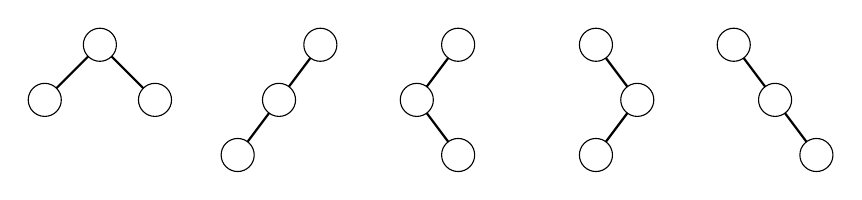
\begin{tikzpicture}[scale=0.7]
\path[draw,thick,-] (0,0) -- (-1,-1);
\path[draw,thick,-] (0,0) -- (1,-1);
\draw[fill=white] (0,0) circle (0.3);
\draw[fill=white] (-1,-1) circle (0.3);
\draw[fill=white] (1,-1) circle (0.3);

\path[draw,thick,-] (4,0) -- (4-0.75,-1) -- (4-1.5,-2);
\draw[fill=white] (4,0) circle (0.3);
\draw[fill=white] (4-0.75,-1) circle (0.3);
\draw[fill=white] (4-1.5,-2) circle (0.3);

\path[draw,thick,-] (6.5,0) -- (6.5-0.75,-1) -- (6.5-0,-2);
\draw[fill=white] (6.5,0) circle (0.3);
\draw[fill=white] (6.5-0.75,-1) circle (0.3);
\draw[fill=white] (6.5-0,-2) circle (0.3);

\path[draw,thick,-] (9,0) -- (9+0.75,-1) -- (9-0,-2);
\draw[fill=white] (9,0) circle (0.3);
\draw[fill=white] (9+0.75,-1) circle (0.3);
\draw[fill=white] (9-0,-2) circle (0.3);

\path[draw,thick,-] (11.5,0) -- (11.5+0.75,-1) -- (11.5+1.5,-2);
\draw[fill=white] (11.5,0) circle (0.3);
\draw[fill=white] (11.5+0.75,-1) circle (0.3);
\draw[fill=white] (11.5+1.5,-2) circle (0.3);
\end{tikzpicture}
\end{center}
және төмендегідей түбірлі дарақтар болады
% and the rooted trees are
\begin{center}
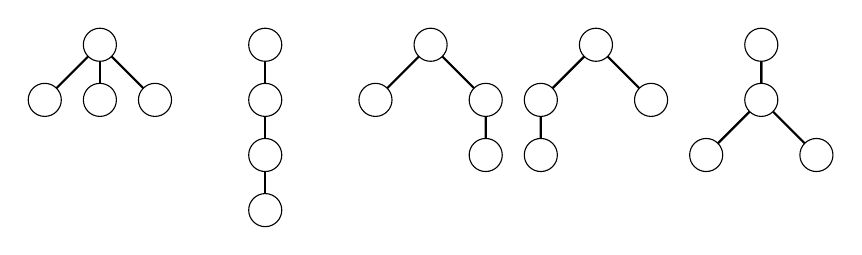
\begin{tikzpicture}[scale=0.7]
\path[draw,thick,-] (0,0) -- (-1,-1);
\path[draw,thick,-] (0,0) -- (0,-1);
\path[draw,thick,-] (0,0) -- (1,-1);
\draw[fill=white] (0,0) circle (0.3);
\draw[fill=white] (-1,-1) circle (0.3);
\draw[fill=white] (0,-1) circle (0.3);
\draw[fill=white] (1,-1) circle (0.3);

\path[draw,thick,-] (3,0) -- (3,-1) -- (3,-2) -- (3,-3);
\draw[fill=white] (3,0) circle (0.3);
\draw[fill=white] (3,-1) circle (0.3);
\draw[fill=white] (3,-2) circle (0.3);
\draw[fill=white] (3,-3) circle (0.3);

\path[draw,thick,-] (6+0,0) -- (6-1,-1);
\path[draw,thick,-] (6+0,0) -- (6+1,-1) -- (6+1,-2);
\draw[fill=white] (6+0,0) circle (0.3);
\draw[fill=white] (6-1,-1) circle (0.3);
\draw[fill=white] (6+1,-1) circle (0.3);
\draw[fill=white] (6+1,-2) circle (0.3);

\path[draw,thick,-] (9+0,0) -- (9+1,-1);
\path[draw,thick,-] (9+0,0) -- (9-1,-1) -- (9-1,-2);
\draw[fill=white] (9+0,0) circle (0.3);
\draw[fill=white] (9+1,-1) circle (0.3);
\draw[fill=white] (9-1,-1) circle (0.3);
\draw[fill=white] (9-1,-2) circle (0.3);

\path[draw,thick,-] (12+0,0) -- (12+0,-1) -- (12-1,-2);
\path[draw,thick,-] (12+0,0) -- (12+0,-1) -- (12+1,-2);
\draw[fill=white] (12+0,0) circle (0.3);
\draw[fill=white] (12+0,-1) circle (0.3);
\draw[fill=white] (12-1,-2) circle (0.3);
\draw[fill=white] (12+1,-2) circle (0.3);

\end{tikzpicture}
\end{center}

\section{Inclusion–exclusion principle} % TODO

\index{inclusion–exclusion principle}


\key{Inclusion–exclusion principle} -- жиындар қиылысуының өлшемі берілген кездегі  
жиындар біріктіруінің өлшемін есептеуге арналған техника. % TODO add kerisinwe
Төмендегі формула аталмыш техникаға қарапайым мысал бола алады:
\[ |A \cup B| = |A| + |B| - |A \cap B|,\]
мұнда $A$ мен $B$ жиындар және $|X|$ деп 
$X$-тің өлшемін белгілейміз. 
Формула төмендегідей көрініс алады:

% \key{Inclusion-exclusion} is a technique
% that can be used for counting the size
% of a union of sets when the sizes of
% the intersections are known, and vice versa.
% A simple example of the technique is the formula
% \[ |A \cup B| = |A| + |B| - |A \cap B|,\]
% where $A$ and $B$ are sets and $|X|$
% denotes the size of $X$.
% The formula can be illustrated as follows:

\begin{center}
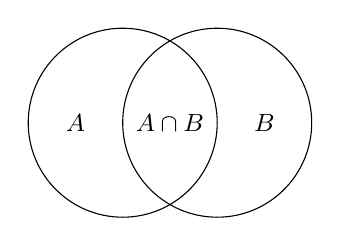
\begin{tikzpicture}[scale=0.8]

\draw (0,0) circle (1.5);
\draw (1.5,0) circle (1.5);

\node at (-0.75,0) {\small $A$};
\node at (2.25,0) {\small $B$};
\node at (0.75,0) {\small $A \cap B$};

\end{tikzpicture}
\end{center}

Біздің мақсатымыз -- кем дегенде бір шеңберге кіретін бөліктің ауданына қатысты $A \cup B$ біріктіруін 
есептеу. 
Сурет $A \cup B$ ауданын есептеу үшін алдымен $A$ мен $B$-ның ауданының
қосындысын тауып, $A \cap B$ ауданын азайтса болатынын көрсетеді.

% Our goal is to calculate
% the size of the union $A \cup B$
% that corresponds to the area of the region
% that belongs to at least one circle.
% The picture shows that we can calculate
% the area of $A \cup B$ by first summing the
% areas of $A$ and $B$ and then subtracting
% the area of $A \cap B$.

Дәл осындай идеяны жиындардың саны көп болған кезде де
қолдануға болады.
Егер үш жиын болса, inclusion–exclusion формуласы % TODO
\[ |A \cup B \cup C| = |A| + |B| + |C| - |A \cap B|  - |A \cap C|  - |B \cap C| + |A \cap B \cap C| \]
және оған сәйкес сурет төмендегідей болады:

% The same idea can be applied when the number
% of sets is larger.
% When there are three sets, the inclusion-exclusion formula is
% \[ |A \cup B \cup C| = |A| + |B| + |C| - |A \cap B|  - |A \cap C|  - |B \cap C| + |A \cap B \cap C| \]
% and the corresponding picture is

\begin{center}
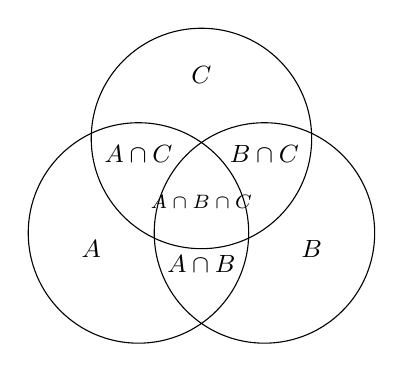
\begin{tikzpicture}[scale=0.8]

\draw (0,0) circle (1.75);
\draw (2,0) circle (1.75);
\draw (1,1.5) circle (1.75);

\node at (-0.75,-0.25) {\small $A$};
\node at (2.75,-0.25) {\small $B$};
\node at (1,2.5) {\small $C$};
\node at (1,-0.5) {\small $A \cap B$};
\node at (0,1.25) {\small $A \cap C$};
\node at (2,1.25) {\small $B \cap C$};
\node at (1,0.5) {\scriptsize $A \cap B \cap C$};

\end{tikzpicture}
\end{center}

Жалпы жағдайда $X_1 \cup X_2 \cup \cdots \cup X_n$ біріктіруінің 
өлшемін $X_1,X_2,\ldots,X_n$ жиындардың барлық қиылысуларынан өтіп санасақ болады. Егер жиындардың саны тақ болса, онда қиылысуын жауапқа қосатын 
боламыз. Басқаша жағдайда қиылысуын жауаптан шегереміз. 

% In the general case, the size of the 
% union $X_1 \cup X_2 \cup \cdots \cup X_n$
% can be calculated by going through all possible
% intersections that contain some of the sets $X_1,X_2,\ldots,X_n$.
% If the intersection contains an odd number of sets,
% its size is added to the answer,
% and otherwise its size is subtracted from the answer.

Осыған ұқсас формуланы жиындардың 
біріктірулерінің өлшемдері арқылы жиындардың 
қиылысуының өлшемін табуға қолдана алатынымызды ескеру керек.
Мысалы
\[ |A \cap B| = |A| + |B| - |A \cup B|\]
және 
\[ |A \cap B \cap C| = |A| + |B| + |C| - |A \cup B|  - |A \cup C|  - |B \cup C| + |A \cup B \cup C| .\]

% Note that there are similar formulas
% for calculating
% the size of an intersection from the sizes of
% unions. For example,
% \[ |A \cap B| = |A| + |B| - |A \cup B|\]
% and
% \[ |A \cap B \cap C| = |A| + |B| + |C| - |A \cup B|  - |A \cup C|  - |B \cup C| + |A \cup B \cup C| .\]

\subsubsection{Ретсіздіктер}

\index{ретсіздіктер}

Өрнек ретінде $\{1,2,\ldots,n\}$ элементтерінің \key{ретсіздіктерін}, яғни ешқандай элемент өз орында тұрмайтын алмастыруларды санайық.
Мысалы,  $n=3$ болғанда, екі ретсіздік кездеседі. олар: $(2,3,1)$ және $(3,1,2)$.

% As an example, let us count the number of \key{derangements}
% of elements $\{1,2,\ldots,n\}$, i.e., permutations
% where no element remains in its original place.
% For example, when $n=3$, there are
% two derangements: $(2,3,1)$ and $(3,1,2)$.

Бұл есептің шығару жолдарының бірі -- inclusion–exclusion әдісін қолдану. % TODO
$X_k$ деп $k$ элементі $k$-позициясында тұратын алмастыруларды белгілейік.
Мысалы $n=3$ болған кезде төмендегідей жиындар құрылады:
\[
\begin{array}{lcl}
X_1 & = & \{(1,2,3),(1,3,2)\} \\
X_2 & = & \{(1,2,3),(3,2,1)\} \\
X_3 & = & \{(1,2,3),(2,1,3)\} \\
\end{array}
\]
Осы жиындарды қолданып отырғандағы ретсіздіктер саны --
\[ n! - |X_1 \cup X_2 \cup \cdots \cup X_n|, \]
демек бізге жиындардың біріктіруінің өлшемін табу жеткілікті.
Inclusion–exclusion әдісін пайдалансақ, бұл есепті қиылысулардың
өлшемін табу есебіне келтіре аламыз. Ал ол болса,
тиімді түрде есептелінеді. Мысалы $n=3$ болған кезде
$|X_1 \cup X_2 \cup X_3|$-нің өлшемі 
\[
\begin{array}{lcl}
 & & |X_1| + |X_2| + |X_3| - |X_1 \cap X_2|  - |X_1 \cap X_3|  - |X_2 \cap X_3| + |X_1 \cap X_2 \cap X_3| \\
 & = & 2+2+2-1-1-1+1 \\
 & = & 4, \\
\end{array}
\]
демек жауаптардың саны -- $3!-4=2$.

% One approach for solving the problem is to use
% inclusion-exclusion.
% Let $X_k$ be the set of permutations
% that contain the element $k$ at position $k$.
% For example, when $n=3$, the sets are as follows:
% \[
% \begin{array}{lcl}
% X_1 & = & \{(1,2,3),(1,3,2)\} \\
% X_2 & = & \{(1,2,3),(3,2,1)\} \\
% X_3 & = & \{(1,2,3),(2,1,3)\} \\
% \end{array}
% \]
% Using these sets, the number of derangements equals
% \[ n! - |X_1 \cup X_2 \cup \cdots \cup X_n|, \]
% so it suffices to calculate the size of the union.
% Using inclusion-exclusion, this reduces to
% calculating sizes of intersections which can be
% done efficiently.
% For example, when $n=3$, the size of
% $|X_1 \cup X_2 \cup X_3|$ is
% \[
% \begin{array}{lcl}
%  & & |X_1| + |X_2| + |X_3| - |X_1 \cap X_2|  - |X_1 \cap X_3|  - |X_2 \cap X_3| + |X_1 \cap X_2 \cap X_3| \\
%  & = & 2+2+2-1-1-1+1 \\
%  & = & 4, \\
% \end{array}
% \]
% so the number of solutions is $3!-4=2$.

Есепті inclusion–exclusion-сіз де шығаруға болады екен. 
$f(n)$ деп $\{1,2,\ldots,n\}$ элементтерінің ретсіздік санын белгілейік. 
Келесі рекурсивті формула арқылы оны есептеуге болады:

% It turns out that the problem can also be solved
% without using inclusion-exclusion.
% Let $f(n)$ denote the number of derangements
% for $\{1,2,\ldots,n\}$. We can use the following
% recursive formula:

\begin{equation*}
    f(n) = \begin{cases}
               0               & n = 1\\
               1               & n = 2\\
               (n-1)(f(n-2) + f(n-1)) & n>2 \\
           \end{cases}
\end{equation*}

Формуланы 1-элементтің ретсіздікті қалай өзгертетінін қарастыру арқылы
дәлелдесек болады. 1-элементтің орынында тұратын $x$ элементін $n-1$ жолмен
таңдасақ болады. Әр жағдайдың екі нұсқасы болады:

% The formula can be derived by considering
% the possibilities how the element 1 changes
% in the derangement.
% There are $n-1$ ways to choose an element $x$
% that replaces the element 1.
% In each such choice, there are two options:

\textit{1–нұсқа:} $x$ элементі 1-элементпен орын алмасады.
Осыдан кейін $n-2$ элементтен тұратын ретсіздіктер санын санау ғана
қалады. 

% \textit{Option 1:} We also replace the element $x$
% with the element 1.
% After this, the remaining task is to construct
% a derangement of $n-2$ elements.

\textit{2-нұсқа:} $x$ элементін 1-элементтен басқа 
элементпен ауыстырамыз. Енді бізге $n-1$ элементтен
тұратын ретсіздіктерді құрастыру қажет болады. Өйткені біз
$x$ элементін 1-элементпен ауыстыра алмаймыз және
қалған басқа элементтер де өзгеруі қажет болады. 

% \textit{Option 2:} We replace the element $x$
% with some other element than 1.
% Now we have to construct a derangement
% of $n-1$ element, because we cannot replace
% the element $x$ with the element $1$, and all other
% elements must be changed.

\section{Бернсайд леммасы}

\index{Бернсайд леммасы}

\key{Бернсайд леммасын} 
әр симметрикалық комбинацияларды тек бір рет 
санау арқылы комбинацияларды есептеуге қолдануға болады. 
Бернсайд леммасы комбинациялар саны 
\[\sum_{k=1}^n \frac{c(k)}{n}\]
екенін тұжырымдайды, мұндағы $n$ -- 
комбинациянының орындарын ауыстыру жолдарының саны, ал
$c(k)$ -- $k$-нші ауыстыру жолын қолданғандағы
өзгермеген комбинациялар саны. 

% \key{Burnside's lemma}
% %\footnote{Actually, Burnside did not discover this lemma; he only mentioned it in his book \cite{bur97}.}
% can be used to count
% the number of combinations so that
% only one representative is counted
% for each group of symmetric combinations.
% Burnside's lemma states that the number of
% combinations is
% \[\sum_{k=1}^n \frac{c(k)}{n},\]
% where there are $n$ ways to change the
% position of a combination,
% and there are $c(k)$ combinations that
% remain unchanged when the $k$th way is applied.

Өрнек ретінде $n$ тастан тұратын және әр таста 
$m$ түс бола алатын алқалардың санын есептейік. 
Екі алқа, егер оларды айналдырғаннан 
кейін ұқсас бола берсе, симметриялы болады.
Мысалы төмендегі алқаға
% As an example, let us calculate the number of
% necklaces of $n$ pearls,
% where each pearl has $m$ possible colors.
% Two necklaces are symmetric if they are
% similar after rotating them.
% For example, the necklace
\begin{center}
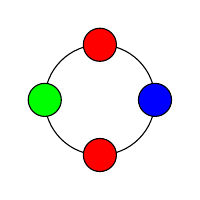
\begin{tikzpicture}[scale=0.7]
\draw[fill=white] (0,0) circle (1);
\draw[fill=red] (0,1) circle (0.3);
\draw[fill=blue] (1,0) circle (0.3);
\draw[fill=red] (0,-1) circle (0.3);
\draw[fill=green] (-1,0) circle (0.3);
\end{tikzpicture}
\end{center} 
келесі симметриялы алқалар болады:
% has the following symmetric necklaces:
\begin{center}
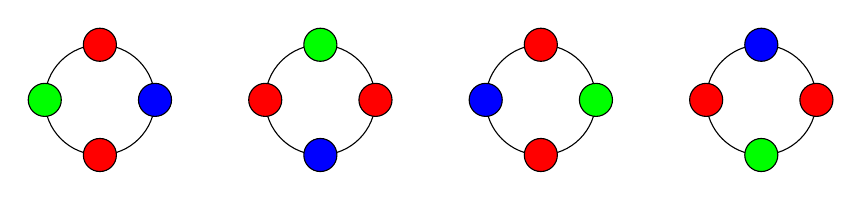
\begin{tikzpicture}[scale=0.7]
\draw[fill=white] (0,0) circle (1);
\draw[fill=red] (0,1) circle (0.3);
\draw[fill=blue] (1,0) circle (0.3);
\draw[fill=red] (0,-1) circle (0.3);
\draw[fill=green] (-1,0) circle (0.3);

\draw[fill=white] (4,0) circle (1);
\draw[fill=green] (4+0,1) circle (0.3);
\draw[fill=red] (4+1,0) circle (0.3);
\draw[fill=blue] (4+0,-1) circle (0.3);
\draw[fill=red] (4+-1,0) circle (0.3);

\draw[fill=white] (8,0) circle (1);
\draw[fill=red] (8+0,1) circle (0.3);
\draw[fill=green] (8+1,0) circle (0.3);
\draw[fill=red] (8+0,-1) circle (0.3);
\draw[fill=blue] (8+-1,0) circle (0.3);

\draw[fill=white] (12,0) circle (1);
\draw[fill=blue] (12+0,1) circle (0.3);
\draw[fill=red] (12+1,0) circle (0.3);
\draw[fill=green] (12+0,-1) circle (0.3);
\draw[fill=red] (12+-1,0) circle (0.3);
\end{tikzpicture}
\end{center}

Алқа позициясын өзгеруінің $n$ жолы бар:
$0,1,\ldots,n-1$ рет сағат бағыты бойынша айналдыруға 
болады. 0 айналдырудан кейін
$m^n$ алқалар өзгермейді. 1 айналдырудан кейін тастарының 
түстері бірдей болатын $m$ алқалар ғана өзгермейді. 

% There are $n$ ways to change the position
% of a necklace,
% because we can rotate it
% $0,1,\ldots,n-1$ steps clockwise.
% If the number of steps is 0,
% all $m^n$ necklaces remain the same,
% and if the number of steps is 1,
% only the $m$ necklaces where each
% pearl has the same color remain the same.

Жалпылай айтқанда, айналдыру саны $k$ болса, 
\[m^{\textrm{gcd}(k,n)}\]
алқалар өзгермейді, мұндағы $\textrm{gcd}(k,n)$
-- $k$ мен $n$-нің ең үлкен ортақ бөлгіші. Өйткені
ұзындығы $\textrm{gcd}(k,n)$ болатын алқаның бөліктері
орындарын ауыстырады. Осылайша Бернсайд леммасы бойынша
алқалардың жалпы саны --
\[\sum_{i=0}^{n-1} \frac{m^{\textrm{gcd}(i,n)}}{n}. \]
Мысалы, егер алқаның ұзындығы 4 және тастардың түстерінің саны
3 болса, алқалардың саны --
\[\frac{3^4+3+3^2+3}{4} = 24. \]

% More generally, when the number of steps is $k$,
% a total of
% \[m^{\textrm{gcd}(k,n)}\]
% necklaces remain the same,
% where $\textrm{gcd}(k,n)$ is the greatest common
% divisor of $k$ and $n$.
% The reason for this is that blocks
% of pearls of size $\textrm{gcd}(k,n)$
% will replace each other.
% Thus, according to Burnside's lemma,
% the number of necklaces is
% \[\sum_{i=0}^{n-1} \frac{m^{\textrm{gcd}(i,n)}}{n}. \]
% For example, the number of necklaces of length 4
% with 3 colors is
% \[\frac{3^4+3+3^2+3}{4} = 24. \]

\section{Кели теоремасы}

\index{Кели теоремасы}

\key{Кели теоремасы} 
$n$ төбеден тұратын және сандармен белгіленген
$n^{n-2}$ дарақтың бар екенін тұжырымдайды. Төбелер 
$1,2,\ldots,n$ сандарымен белгіленеді. 
Егер 
құрылымдары немесе белгіленген сандары бірдей болмаса, екі дарақ бірдей емес деп есептеледі.

% \key{Cayley's formula}
% % \footnote{While the formula is named after A. Cayley,
% % who studied it in 1889, it was discovered earlier by C. W. Borchardt in 1860.}
% states that
% there are $n^{n-2}$ labeled trees
% that contain $n$ nodes.
% The nodes are labeled $1,2,\ldots,n$,
% and two trees are different
% if either their structure or
% labeling is different.

\begin{samepage}
Мысалы $n=4$ болған кезде, сандармен белгіленген $4^{4-2}=16$ дарақ болады:
% For example, when $n=4$, the number of labeled
% trees is $4^{4-2}=16$:

\begin{center}
\begin{tikzpicture}[scale=0.8]
\footnotesize

\newcommand\puua[6]{
\path[draw,thick,-] (#1,#2) -- (#1-1.25,#2-1.5);
\path[draw,thick,-] (#1,#2) -- (#1,#2-1.5);
\path[draw,thick,-] (#1,#2) -- (#1+1.25,#2-1.5);
\node[draw, circle, fill=white] at (#1,#2) {#3};
\node[draw, circle, fill=white] at (#1-1.25,#2-1.5) {#4};
\node[draw, circle, fill=white] at (#1,#2-1.5) {#5};
\node[draw, circle, fill=white] at (#1+1.25,#2-1.5) {#6};
}
\newcommand\puub[6]{
\path[draw,thick,-] (#1,#2) -- (#1+1,#2);
\path[draw,thick,-] (#1+1,#2) -- (#1+2,#2);
\path[draw,thick,-] (#1+2,#2) -- (#1+3,#2);
\node[draw, circle, fill=white] at (#1,#2) {#3};
\node[draw, circle, fill=white] at (#1+1,#2) {#4};
\node[draw, circle, fill=white] at (#1+2,#2) {#5};
\node[draw, circle, fill=white] at (#1+3,#2) {#6};
}

\puua{0}{0}{1}{2}{3}{4}
\puua{4}{0}{2}{1}{3}{4}
\puua{8}{0}{3}{1}{2}{4}
\puua{12}{0}{4}{1}{2}{3}

\puub{0}{-3}{1}{2}{3}{4}
\puub{4.5}{-3}{1}{2}{4}{3}
\puub{9}{-3}{1}{3}{2}{4}
\puub{0}{-4.5}{1}{3}{4}{2}
\puub{4.5}{-4.5}{1}{4}{2}{3}
\puub{9}{-4.5}{1}{4}{3}{2}
\puub{0}{-6}{2}{1}{3}{4}
\puub{4.5}{-6}{2}{1}{4}{3}
\puub{9}{-6}{2}{3}{1}{4}
\puub{0}{-7.5}{2}{4}{1}{3}
\puub{4.5}{-7.5}{3}{1}{2}{4}
\puub{9}{-7.5}{3}{2}{1}{4}
\end{tikzpicture}
\end{center}
\end{samepage}

Кели теоремасын дәлелдеу үшін Прюфер кодтарын
қолдануға болады. 

% Next we will see how Cayley's formula can
% be derived using Prüfer codes.

\subsubsection{Прюфер кодтары}

\index{Прюфер кодтары}

\key{Прюфер коды} --
%\footnote{In 1918, H. Prüfer proved Cayley's theorem using Prüfer codes \cite{pru18}.}
$n-2$ сандардан тұратын белгіленген дарақты сипаттайтын тізбек.
Код дарақтан $n-2$ жапырақтарды өшіру үдерісі арқылы 
құрастырылады. Әр қадамда белгісі ең кіші жапырақ өшіріледі және
оның жалғыз көршісінің белгісі кодқа жазылады.

% A \key{Prüfer code}
% %\footnote{In 1918, H. Prüfer proved Cayley's theorem using Prüfer codes \cite{pru18}.}
% is a sequence of
% $n-2$ numbers that describes a labeled tree.
% The code is constructed by following a process
% that removes $n-2$ leaves from the tree.
% At each step, the leaf with the smallest label is removed,
% and the label of its only neighbor is added to the code.

Мысалы келесі графтың Прюфер кодын есептейік:
% For example, let us calculate the Prüfer code
% of the following graph:
\begin{center}
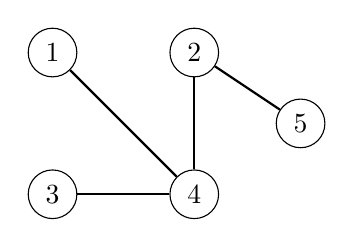
\begin{tikzpicture}[scale=0.9]
\node[draw, circle] (1) at (2,3) {$1$};
\node[draw, circle] (2) at (4,3) {$2$};
\node[draw, circle] (3) at (2,1) {$3$};
\node[draw, circle] (4) at (4,1) {$4$};
\node[draw, circle] (5) at (5.5,2) {$5$};

\path[draw,thick,-] (1) -- (4);
\path[draw,thick,-] (3) -- (4);
\path[draw,thick,-] (2) -- (4);
\path[draw,thick,-] (2) -- (5);
\end{tikzpicture}
\end{center}

Алдымен біз 1-төбені өшіреміз, сосын 4-төбені кодқа қосамыз:
% First we remove node 1 and add node 4 to the code:
\begin{center}
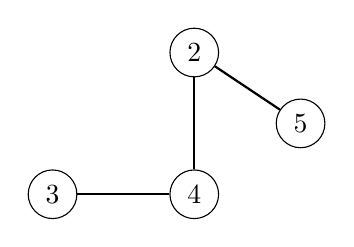
\begin{tikzpicture}[scale=0.9]
%\node[draw, circle] (1) at (2,3) {$1$};
\node[draw, circle] (2) at (4,3) {$2$};
\node[draw, circle] (3) at (2,1) {$3$};
\node[draw, circle] (4) at (4,1) {$4$};
\node[draw, circle] (5) at (5.5,2) {$5$};

%\path[draw,thick,-] (1) -- (4);
\path[draw,thick,-] (3) -- (4);
\path[draw,thick,-] (2) -- (4);
\path[draw,thick,-] (2) -- (5);
\end{tikzpicture}
\end{center}

Кейін 3-төбені өшіреміз және 4-төбені кодқа қосамыз:
% Then we remove node 3 and add node 4 to the code:
\begin{center}
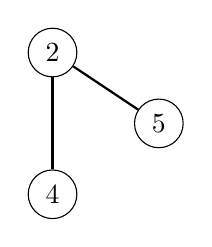
\begin{tikzpicture}[scale=0.9]
%\node[draw, circle] (1) at (2,3) {$1$};
\node[draw, circle] (2) at (4,3) {$2$};
%\node[draw, circle] (3) at (2,1) {$3$};
\node[draw, circle] (4) at (4,1) {$4$};
\node[draw, circle] (5) at (5.5,2) {$5$};

%\path[draw,thick,-] (1) -- (4);
%\path[draw,thick,-] (3) -- (4);
\path[draw,thick,-] (2) -- (4);
\path[draw,thick,-] (2) -- (5);
\end{tikzpicture}
\end{center}

Соңында 4-төбені өшіріп, 2-төбені кодқа қосамыз:
% Finally we remove node 4 and add node 2 to the code:
\begin{center}
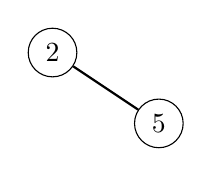
\begin{tikzpicture}[scale=0.9]
%\node[draw, circle] (1) at (2,3) {$1$};
\node[draw, circle] (2) at (4,3) {$2$};
%\node[draw, circle] (3) at (2,1) {$3$};
%\node[draw, circle] (4) at (4,1) {$4$};
\node[draw, circle] (5) at (5.5,2) {$5$};

%\path[draw,thick,-] (1) -- (4);
%\path[draw,thick,-] (3) -- (4);
%\path[draw,thick,-] (2) -- (4);
\path[draw,thick,-] (2) -- (5);
\end{tikzpicture}
\end{center}

Осылайша дарақтың Прюфер коды $[4,4,2]$-ке тең болады.
% Thus, the Prüfer code of the graph is $[4,4,2]$.

Кез келген дараққа Прюфер кодын құрастыруға болады
және ең маңыздысы, Прюфер кодымен бастапқы дарақты
қайта құра аламыз. Демек $n$ төбеден тұратын 
белгіленген дарақтардың саны $n^{n-2}$-ге, яғни
өлшемі $n$ болатын Прюфер кодтарының санына тең болады. 

% We can construct a Prüfer code for any tree,
% and more importantly,
% the original tree can be reconstructed
% from a Prüfer code.
% Hence, the number of labeled trees
% of $n$ nodes equals
% $n^{n-2}$, the number of Prüfer codes
% of size $n$.
